\documentclass[22pt]{article} 
\usepackage{geometry} 
\usepackage{float} 
\usepackage{graphicx}
\usepackage{caption}
\usepackage{subfigure}
\usepackage{amsmath}
\usepackage{array}
\usepackage{amsfonts}
\geometry{left=2.0cm,right=2.0cm,top=0.5cm,bottom=2cm}
	\author{Mengfan Wang} 
	\title{Stochastic Signal Systems Homework 3} 
\begin{document}
		\maketitle 
	\paragraph{1}
		\subparagraph{a}\begin{figure}[H]
				\centering
				\subfigure{
					\begin{minipage}{9cm}
					\centering
					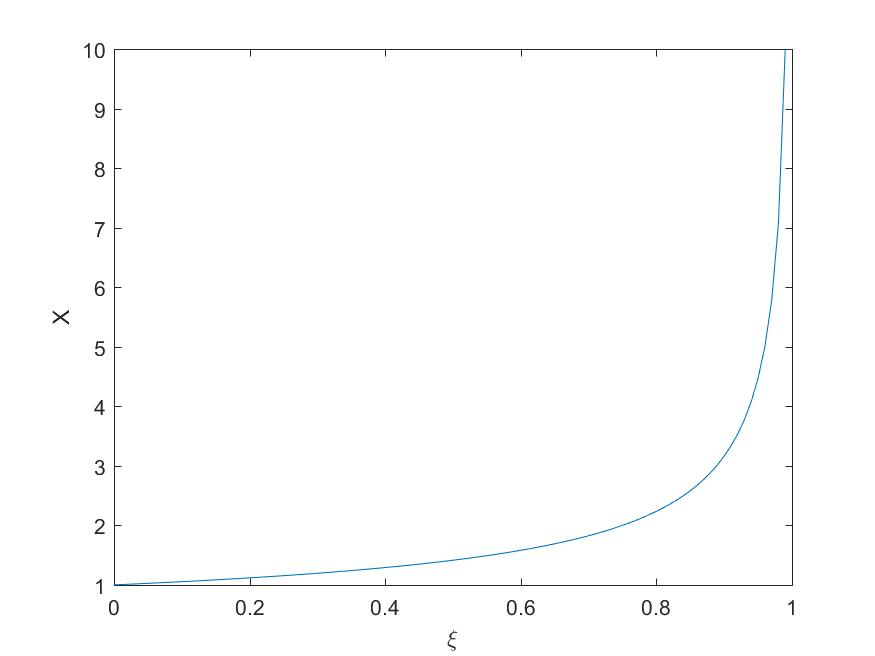
\includegraphics[height=6cm]{1.jpg}
					\end{minipage}
				}
			\end{figure}

		\subparagraph{b} \begin{align}
		F_X(x) & = P[X\leq x]\\
		& = P[\frac{1}{\sqrt{1- \xi}}\leq x]\\
		& = P[1- \xi \geq \frac{1}{x^2}]\\
		& = P[\xi \leq 1-\frac{1}{x^2}]\\
		& = 1 -\frac{1}{x^2}
		\end{align}
		So, \begin{align}
	F_X(x) = 
				\begin{cases}
				1 -\frac{1}{x^2} & x \geq 1\\
				0 & otherwise
				\end{cases}
	\end{align}
		\subparagraph{c}
		\begin{align}
		P[X>1] = 1 -F_X(1) = 1 - (1-1) = 1
		\end{align}
		\begin{align}
		P[5<X<7] = F_X(7) - F_X(5^-) = 1/25-1/49 = 24/1225
		\end{align}

	\paragraph{2} We have $X = \frac{Y-b}{a}$, then 
	\begin{align}
	f_Y(y) & = f_X(x)|\frac{dx}{dy}|_{x = \frac{y-b}{a}}\\
		   & = f_X(\frac{y-b}{a})/a\\
		   & = \frac{1}{\sqrt{2 \pi}a}exp(-\frac{(y-b)^2}{2a^2})
	\end{align}
	So $Y$ a Gaussian random variable with mean $b$ and standard deviation $a$.

	\paragraph{3}From the pdf of $X$ we know that $P[X\leq 0||X>0] = 0$. When $0<X\leq 1$, we have $0< Y = \sqrt{X} \leq 1$:
	\begin{align}
	f_Y(y) & = f_X(x)|\frac{dx}{dy}|_{x = y^2}\\
	& = \frac{1}{2y}2y\\
	& = 1
	\end{align}
	So, \begin{align}
	f_Y(y) = 
				\begin{cases}
				1 & 0< y \leq 1\\
				0 & otherwise
				\end{cases}
	\end{align}

	\paragraph{4}It's easy to know $Y \geq 0$: 
	\begin{align}
	f_Y(y) & = f_X(x)|\frac{dx}{dy}|_{x = y} + f_X(x)|\frac{dx}{dy}|_{x = -\sqrt{y}}\\
	& = \frac{1}{\sqrt{2 \pi}}exp(-\frac{y^2}{2}) +  \frac{1}{2\sqrt{2 \pi y}}exp(-\frac{y}{2})
	\end{align}
	So,\begin{align}
	f_Y(y) = 
				\begin{cases}
				\frac{1}{\sqrt{2 \pi}}exp(-\frac{y^2}{2}) +  \frac{1}{2\sqrt{2 \pi y}}exp(-\frac{y}{2}) & y \geq 0\\
				0 & y<0
				\end{cases}
	\end{align}

	\paragraph{5}
	\begin{align} p_Y(0) = P[Y = 0] = P[-1 \leq X \leq 1] = \Phi(\frac{1}{3}) - \Phi(-\frac{1}{3})
	\end{align}
	\begin{align}
	p_Y(0.5) = p_Y(-0.5) = P[1<X \leq 2] = \Phi(\frac{2}{3}) - \Phi(\frac{1}{3})
	\end{align}
	\begin{align} p_Y(1) = p_Y(-1) = P[X>2] = 1 - \Phi(\frac{2}{3})
	\end{align}
	So,\begin{align}
	p_Y(y) = 
				\begin{cases}
				\Phi(\frac{1}{3}) - \Phi(-\frac{1}{3}) & y = 0\\
				\Phi(\frac{2}{3}) - \Phi(\frac{1}{3}) & y = \pm 0.5\\
				1 - \Phi(\frac{2}{3}) & y = \pm 1
				\end{cases}
	\end{align}

	\paragraph{6} $X = \ln Y$, so:
	\begin{align}
	f_Y(y) & = f_X(x)|\frac{dx}{dy}|_{x = \ln y}\\
	& = \frac{1}{\sqrt{2 \pi}\sigma y}exp(-\frac{(\ln y-m)^2}{2 \sigma^2})
	\end{align}

	\paragraph{7} When $0 < X \leq \pi/2$, $X = \arcsin(Y)$; when $\pi/2 <X<\pi$, $X =\pi- \arcsin(Y)$. So,
	\begin{align}
	f_Y(y) & = f_X(x)|\frac{dx}{dy}|_{x = \arcsin(y)}+ f_X(x)|\frac{dx}{dy}|_{x = \pi-\arcsin(y)}\\
	& = \frac{2}{\pi\sqrt{1-y^2}}
	\end{align}\
	So, \begin{align}
	f_Y(y) = 
				\begin{cases}
				\frac{2}{\pi\sqrt{1-y^2}} & 0<y\leq1\\
				0 & otherwise
				\end{cases}
	\end{align}

	\paragraph{8} $P[X>b] = P[X < b] = 1-\Phi(1)$.
	When $-b\leq x \leq b$, $f_Y(y) = f_X(x)$.
	So,\begin{align}
	f_Y(y) = 
				\begin{cases}
				 \frac{1}{\sqrt{2 \pi }b}exp(-\frac{y^2}{2b^2}) + (1-\Phi(1))(\delta(y-b)+\delta(y+b) )  & -b\leq y \leq b\\
				 0 & otherwise
				\end{cases}
	\end{align}

	\paragraph{9} When $0\leq x <1$, $x = \sqrt{y}$; When $-1<x<0$,$x = -\sqrt{y}$.
	\begin{align}
	f_Y(y) & = f_X(x)|\frac{dx}{dy}|_{x = \sqrt{y}} + f_X(x)|\frac{dx}{dy}|_{x = -\sqrt{y}}\\
	& = \frac{1}{4\sqrt{y}} + \frac{1}{2}\delta(y-\frac{1}{16})
	\end{align} 
	So,\begin{align}
	f_Y(y) = 
				\begin{cases}
				 \frac{1}{4\sqrt{y}} + \frac{1}{2}\delta(y-\frac{1}{16}) & 0\leq x <1\\
				 0 & otherwise,
				\end{cases}
	\end{align}
	And,\begin{align}
	F_Y(y) = 
				\begin{cases}
				 0 & y <0\\
				\frac{\sqrt{y}}{2} & 0\leq y<\frac{1}{16}\\
				\frac{\sqrt{y}}{2} + \frac{1}{2} & \frac{1}{16} \leq y \leq 1\\
				 1 & y>1
				\end{cases}
	\end{align}

	\paragraph{10}
	\begin{align}
	E[X] & = \sum_{k=0}^{\infty}k\frac{a^k}{k!}e^{-a}\\
	& = e^{-a}a\sum_{k=0}^{\infty}\frac{a^{k-1}}{(k-1)!}\\
	& = a
	\end{align}

	\begin{align}
	VAR[X] & = E[X^2] -E[X]^2\\
	& = \sum_{k=0}^{\infty}k^2\frac{a^k}{k!}e^{-a} - a^2\\
	& = e^{-a}\sum_{k=0}^{\infty}\frac{(k-1+1)a^k}{(k-1)!} - a^2\\
	& = e^{-a}(\sum_{k=0}^{\infty}\frac{a^k}{(k-1)!}+\sum_{k=0}^{\infty}\frac{a^k}{(k-2)!}) - a^2\\
	& = e^{-a}(ae^a+a^2e^a)-a^2\\
	& = a
	\end{align}

	\paragraph{11}
	\begin{align}
	E[X^n] = \int_0^1 x^ndx = \frac{x^{n+1}}{n+1}|_1 - \frac{x^{n+1}}{n+1}|_0 = \frac{1}{n+1}
	\end{align}
	\begin{align}
	E[X^n] = \int_a^b x^n\frac{1}{b-a}dx = \frac{1}{b-a}(\frac{x^{n+1}}{n+1}|_b - \frac{x^{n+1}}{n+1}|_a) = \frac{1}{b-a}\frac{b^{n+1}-a^{n+1}}{n+1}
	\end{align}

	\paragraph{12}
	\begin{align}
	E[X] & = \int_0^\infty x \lambda	e^{-\lambda	x}dx\\
	& = \frac{1}{\lambda}\int_0^\infty x \lambda^2 e^{-\lambda	x}dx\\
	& = \frac{1}{\lambda}[(-e^{-\lambda	x}-\lambda	xe^{-\lambda x})|_\infty - (-e^{-\lambda	x}-\lambda	xe^{-\lambda x})|_0]\\
	& = \frac{1}{\lambda}
	\end{align}

	\paragraph{13}
		\subparagraph{a} \begin{align}E[X] = \frac{1}{8}\sum_{k=-3}^{4}k = \frac{1}{2}
		\end{align}
		\begin{align}
		VAR[X] = E[X^2]-E[X]^2 = \frac{1}{8}\sum_{k=-3}^{4}k^2 - \frac{1}{4} = \frac{21}{4}
		\end{align}
		\subparagraph{b} \begin{align}E[Y] = -2E[X^2]+3 = -8
		\end{align}
		\begin{align}VAR[Y] = E[Y^2]-E[Y]^2 = \frac{1}{8}\sum_{k=-3}^{4}(-2k^2+3) -E[Y]^2 =  105
		\end{align}



\end{document}